\chapter{Elektromagnetische inductie en toepassingen}\label{ch:b1:induction}

Beweeg een magneet naar een spoel toe en er loopt een stroom in de spoel; stop de
magneet en de stroom stopt. Faraday vond dit in 1831, na tien
jaar zoeken, en het is het feit waarop de elektrische wereld
draait: elke elektriciteitscentrale, elke transformator, elke motor en
luidspreker en microfoon, elke inductiekookplaat en draadloze
lader zet energie om via de wet dat een \emph{veranderende} \omterm{def:b1:induction:flux}{magnetische
flux} een elektromotorische \omterm{def:b1:dc-circuits:voltage}{spanning} aandrijft. Dit hoofdstuk formuleert de wet met
haar tekens, geeft haar de twee gedaanten die zij aanneemt (een veranderend veld in een vaste
kring, een kring die in een vast veld beweegt), definieert zelf- en \omterm{def:b1:induction:inductance}{wederzijdse
inductie}, en werkt daarna de elektromechanische machines uit ---
de schuivende staaf, de alternator, de transformator, de luidspreker ---
waar dezelfde wet mechanisch vermogen in \omterm{thm:b1:dc-circuits:kirchhoff}{elektrisch vermogen} omzet en
terug, nooit voor niets.

\begin{omfigure}
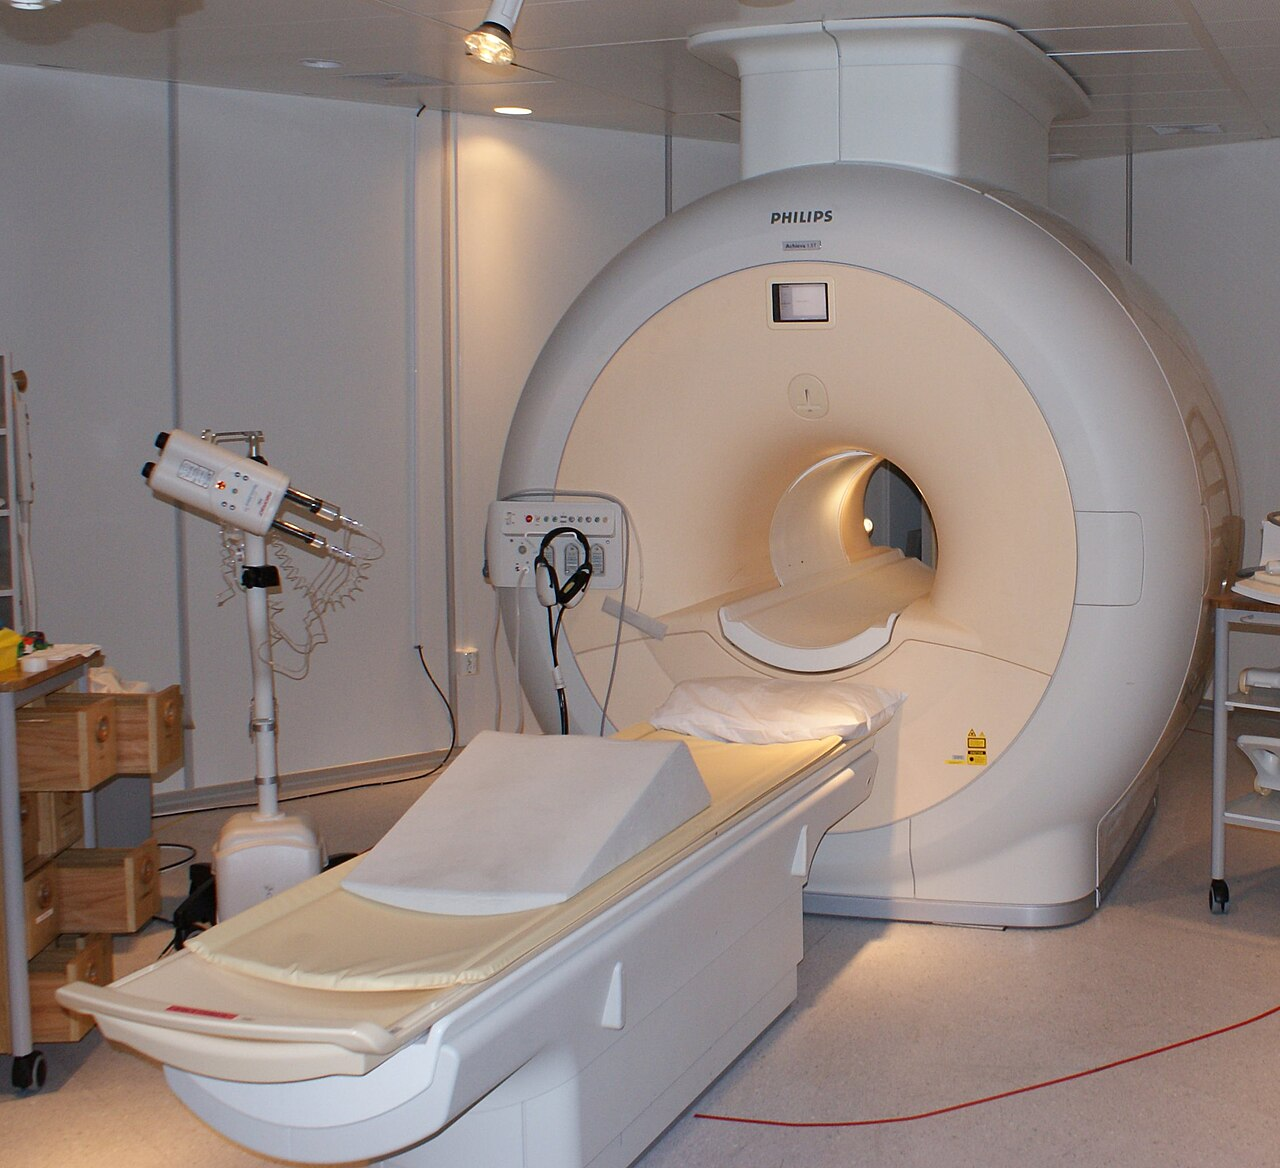
\includegraphics[width=0.50\linewidth]{images/book3/mri-scanner.jpg}

{\small Een MRI-scanner: een supergeleidende spoel die \qty{1.5}{T} boven een patiënt aanhoudt --- een megajoule aan \omterm{prop:b1:induction:inductor}{magnetische energie} in een veld met niets erin. Foto: Jan Ainali, CC~BY~3.0.}
\end{omfigure}

\section{De wet van Faraday}

\begin{definition}[Magnetische flux door een kring]\label{def:b1:induction:flux}
\index{magnetische flux}\index{weber}
Oriënteer een gesloten kring $\Gamma$ (een doorlooprichting); zijn oppervlak krijgt
de normaal $\vect n$ volgens de rechterhandregel. De \emph{magnetische
flux} door de kring is $\Phi = \sum\vect B\cdot\vect n\,\dd S$ over
elk oppervlak met rand $\Gamma$ (weber, $\qty{1}{Wb} = \qty{1}{T.m^2}$) ---
``elk'', omdat de flux van $\vect B$ door een gesloten oppervlak nul is.
Voor een homogeen veld en een vlakke spoel van $N$ windingen met oppervlakte $S$ is $\Phi =
NBS\cos\alpha$, met $\alpha$ de hoek tussen $\vect B$ en $\vect n$.
\end{definition}

\begin{theorem}[De inductiewet van Faraday]\label{thm:b1:induction:faraday}
\index{wet van Faraday}\index{elektromotorische spanning (geïnduceerde)}\index{wet van Lenz}
Telkens wanneer de flux door een kring verandert is de kring de zetel van
een \emph{geïnduceerde elektromotorische \omterm{def:b1:dc-circuits:voltage}{spanning}}
\[
e = -\frac{\dd\Phi}{\dd t} ,
\]
geteld in de oriëntatie van de kring, dat wil zeggen werkend als een ideale
\omterm{def:b1:dc-circuits:sources}{spanningsbron} met emk $e$ in die zin; in een kring met weerstand $R$
drijft zij de stroom $i = e/R$ aan. Het minteken is de \emph{\omterm{thm:b1:induction:faraday}{wet van Lenz}}:
de geïnduceerde stroom loopt zo dat hij de fluxverandering tegenwerkt die
hem opwekt --- zijn eigen veld, en de krachten die hij voelt, verzetten zich tegen de oorzaak.
\end{theorem}
\admitted

\begin{remark}[Twee gedaanten van dezelfde wet]\label{rem:b1:induction:twofaces}
\index{neumann-inductie}\index{lorentz-inductie}
De flux verandert ofwel omdat $\vect B$ in de tijd verandert door een
vaste kring (\emph{\omterm{rem:b1:induction:twofaces}{neumann-inductie}}: transformator, inductiekookplaat)
ofwel omdat de kring beweegt of vervormt in een stationair veld
(\emph{\omterm{rem:b1:induction:twofaces}{lorentz-inductie}}: generator, luidspreker). In het tweede geval
laat de emk zich ook rechtstreeks berekenen: de ladingsdragers van een geleiderelement
$\dd\vect l$ dat met $\vect v$ beweegt voelen de kracht $q\vect v\wedge
\vect B$, gelijkwaardig aan een elektrisch veld $\vect v\wedge\vect B$, zodat
$e = \oint(\vect v\wedge\vect B)\cdot\dd\vect l$ --- en dit stemt altijd overeen
met $-\dd\Phi/\dd t$. De \omterm{thm:b1:induction:faraday}{wet van Faraday} dekt beide; het volume van jaar 2
legt uit waarom de twee mechanismen één formule geven.
\end{remark}

\begin{omfigure}
\begin{tikzpicture}[font=\small, x=1cm, y=1cm, >=Stealth]
  \begin{scope}
    \draw[omThm, very thick, postaction={decorate, decoration={markings, mark=at position 0.25 with {\arrow{>}}, mark=at position 0.75 with {\arrow{>}}}}] (0,0) ellipse (1.4 and 0.5);
    \draw[omDef, thick, ->] (0,0.5) -- (0,1.7) node[right, font=\footnotesize] {$\vect n$};
    \node[omThm, font=\footnotesize] at (1.75,-0.55) {$\Gamma$};
    \foreach \x in {-0.9,-0.3,0.3,0.9} \draw[omProp, ->] (\x,-1.6) -- (\x,1.2);
    \node[omProp, font=\footnotesize] at (1.4,1.05) {$\vect B$};
    \node[font=\footnotesize] at (0,-2.2) {$\Phi = \vect B\cdot\vect n\,S > 0$};
  \end{scope}
  \begin{scope}[xshift=6.2cm]
    \draw[omThm, very thick, postaction={decorate, decoration={markings, mark=at position 0.25 with {\arrow{<}}, mark=at position 0.75 with {\arrow{<}}}}] (0,0) ellipse (1.4 and 0.5);
    \node[omThm, font=\footnotesize] at (1.75,0.6) {$i$};
    % magnet coming down
    \draw[fill=omDef!20, draw=omDef, thick] (-0.4,1.3) rectangle (0.4,2.0); \node[omDef, font=\footnotesize] at (0,1.65) {Z};
    \draw[fill=omThm!20, draw=omThm, thick] (-0.4,2.0) rectangle (0.4,2.7); \node[omThm, font=\footnotesize] at (0,2.35) {N};
    \draw[very thick, ->] (0.8,2.6) -- (0.8,1.7) node[right, font=\footnotesize] {$\vect v$};
    \draw[omProp, ->] (0,1.25) -- (0,0.2) node[right, font=\footnotesize, pos=0.6] {$\vect B$ (magneet)};
    \draw[omDef, ->] (-0.6,-0.1) -- (-0.6,0.9) node[left, font=\footnotesize, pos=0.7] {$\vect B_{\text{ind}}$};
    \node[font=\footnotesize] at (0,-2.2) {naderende magneet: $i$ stoot hem af};
  \end{scope}
  \begin{scope}[xshift=11.8cm]
    \draw[omThm, very thick] (-1.4,-0.5) rectangle (1.4,0.5);
    \draw[omThm, very thick] (0.5,-0.5) -- (0.5,0.5);
    \draw[omDef, very thick, ->] (0.5,0.5) -- (0.5,-0.5);
    \draw[very thick, ->] (0.6,0.75) -- (1.2,0.75) node[above, font=\footnotesize] {$\vect v$};
    \foreach \x in {-1.1,-0.6,-0.1,0.4,0.9} \node[omProp, font=\scriptsize] at (\x,0.0) {$\odot$};
    \node[omProp, font=\footnotesize] at (1.75,0.0) {$\vect B$};
    \draw[omDef, ->, thick] (0.5,0.0) -- (-0.2,0.0); \node[omDef, font=\footnotesize] at (-0.15,-0.3) {$\vect F$};
    \node[font=\footnotesize] at (0,-2.2) {schuivende staaf: flux groeit, $\vect F$ remt};
  \end{scope}
\end{tikzpicture}

{\small Oriëntatie en de \omterm{thm:b1:induction:faraday}{wet van Lenz}. Links: de oriëntatie van de kring
legt $\vect n$ en het teken van $\Phi$ vast. Midden: een magneet die een
ring nadert vergroot de flux; de geïnduceerde stroom wekt een veld op dat dat
van de magneet tegenwerkt en de ring stoot hem af. Rechts: een staaf die op rails schuift in een
veld dat naar de lezer wijst; de flux van de kring groeit, en de
geïnduceerde stroom loopt zo dat de \omterm{thm:b1:magnetostatics:laplace}{laplacekracht} op de staaf haar beweging
tegenwerkt.}
\end{omfigure}

\begin{example}[Ordes van grootte]\label{ex:b1:induction:orders}
Een spoel van $100$ windingen en \qty{10}{cm^2} in het aardveld, in
\qty{0.1}{s} omgeklapt: $\Delta\Phi = 2 \times 100 \times 10^{-3} \times 5 \times 10^{-5} = \qty{1e-5}{Wb}$,
$e \sim \qty{0.1}{mV}$ --- meetbaar met een gevoelige galvanometer, zoals
het aardveld ooit in kaart is gebracht. Dezelfde spoel in de spleet van \qty{1}{T}
van een magneet, er in \qty{0.1}{s} uit getrokken: \qty{1}{V}. Een transformatorspoel van
$1000$ windingen met \qty{1}{T} bij \qty{50}{Hz} over \qty{10}{cm^2}: $e_{\max} =
1000 \times 10^{-3} \times 314 = \qty{314}{V}$ --- de netspanning.
\end{example}

\section{Zelfinductie en wederzijdse inductie}

\begin{definition}[Inductie]\label{def:b1:induction:inductance}
\index{zelfinductie}\index{henry}\index{wederzijdse inductie}
De flux van het eigen veld van een kring door zichzelf is evenredig met zijn
stroom: $\Phi_{\text{eigen}} = Li$, met $L > 0$ zijn \emph{zelfinductie}
(henry, \unit{H}). De flux die kring~1 door kring~2 stuurt is
$\Phi_{1 \to 2} = Mi_1$, en symmetrisch $\Phi_{2 \to 1} = Mi_2$, met $M$
hun \emph{wederzijdse inductie} (het teken ligt vast door de oriëntaties). De
totale flux van kring~1 is dan $\Phi_1 = L_1i_1 + Mi_2$.
\end{definition}

\begin{proposition}[De spoel; de solenoïde]\label{prop:b1:induction:inductor}
\index{spoel}\index{magnetische energie}\index{energiedichtheid van het magnetische veld}
Een kring met \omterm{def:b1:induction:inductance}{zelfinductie} $L$ die een veranderende stroom voert is de zetel van
de emk $e = -L\,\dd i/\dd t$: in de verbruikersconventie is dat de
\omterm{def:b1:dc-circuits:voltage}{spanning} $u = L\,\dd i/\dd t$ van de spoel die sinds
\cref{ch:b1:transient-regimes} wordt gebruikt. Zij slaat de energie $W = \tfrac12Li^2$ op.
Een lange solenoïde met $n$ windingen per meter, lengte $\ell$ en doorsnede $S$,
heeft $L = \mu_0n^2S\ell$; haar opgeslagen energie is $\tfrac12\mu_0n^2I^2S\ell =
\dfrac{B^2}{2\mu_0}\,S\ell$: \omterm{prop:b1:induction:inductor}{magnetische energie} huist in het veld met
dichtheid $B^2/2\mu_0$, precies zoals elektrische energie met $\varepsilon_0E^2/2$.
\end{proposition}

\begin{proof}
Faraday met $\Phi = Li$ en constante $L$. Energie: het vermogen dat de
spoel ontvangt is $ui = Li\,\dd i/\dd t = \dd(\tfrac12Li^2)/\dd t$. Solenoïde:
$B = \mu_0nI$ binnenin, flux $BS$ door elk van de $n\ell$ windingen, dus $\Phi =
\mu_0n^2S\ell I$. De algemene dichtheid wordt aangenomen.
\end{proof}

\begin{example}[Een MRI-magneet]\label{ex:b1:induction:mri}
\qty{1.5}{T} over ongeveer een kubieke meter: $B^2/2\mu_0 = 2.25/2.5 \times 10^{-6} =
\qty{0.9}{MJ/m^3}$ --- de energie van een autoaccu, opgeslagen in lege ruimte.
Bij een spoelstroom van \qty{500}{A} is $L = 2W/I^2 = \qty{7}{H}$. Wordt de
supergeleider plotseling weerstandsvol (een \emph{quench}), dan wordt die megajoule
in seconden warmte en kookt zij honderden liters vloeibaar
helium weg: de magneetkamer heeft er een afvoer voor.
\end{example}

\begin{proposition}[De ideale transformator]\label{prop:b1:induction:transformer}
\index{transformator}
Twee spoelen met $N_1$ en $N_2$ windingen op dezelfde gesloten ijzeren kern,
zodat dezelfde flux $\varphi$ door elke winding gaat, voldoen aan
\[
\frac{u_2}{u_1} = \frac{N_2}{N_1} , \qquad N_1i_1 + N_2i_2 = 0 \quad\text{(geen belastingverliezen, geen magnetiseringsstroom)},
\]
zodat $u_2i_2 = -u_1i_1$: het vermogen dat de primaire opneemt wordt aan de
secundaire geleverd; \omterm{def:b1:dc-circuits:voltage}{spanningen} schalen met de windingsverhouding, stromen
omgekeerd. Het werkt alleen met veranderende stromen.
\end{proposition}

\begin{proof}
$u_1 = N_1\,\dd\varphi/\dd t$ en $u_2 = N_2\,\dd\varphi/\dd t$ (verbruikersconventie
aan beide kanten, oriëntaties langs de gemeenschappelijke flux gekozen): deel ze op elkaar.
De stroombetrekking is de \omterm{thm:b1:magnetostatics:ampere}{stelling van Ampère} op de kern: haar circulatie,
$\mu_0\mu_r$ maal het totale aantal ampèrewindingen, zou de flux moeten
opwekken; voor een ideale kern ($\mu_r \to \infty$) vergt dat een verwaarloosbaar aantal
ampèrewindingen, en dus $N_1i_1 + N_2i_2 = 0$. In deze vorm aangenomen.
\end{proof}

\begin{omfigure}
\begin{tikzpicture}[font=\small, x=1cm, y=1cm, >=Stealth]
  % core
  \draw[omExo!60, line width=9pt] (-2,-1.5) rectangle (2,1.5);
  % primary windings
  \foreach \y in {-0.9,-0.6,...,0.9} \draw[omThm, thick] (-2.35,\y) arc[start angle=90, end angle=-90, x radius=0.18, y radius=0.15];
  \foreach \y in {-0.9,-0.6,...,0.9} \draw[omDef, thick] (2.35,\y) arc[start angle=90, end angle=270, x radius=0.18, y radius=0.15];
  \draw[omThm, thick] (-2.35,0.9) -- (-3.2,0.9) node[left, font=\footnotesize] {$u_1$}; \draw[omThm, thick] (-2.35,-1.2) -- (-3.2,-1.2);
  \draw[omDef, thick] (2.35,0.9) -- (3.2,0.9) node[right, font=\footnotesize] {$u_2$}; \draw[omDef, thick] (2.35,-1.2) -- (3.2,-1.2);
  \node[omThm, font=\footnotesize] at (-2.9,0) {$N_1$}; \node[omDef, font=\footnotesize] at (2.9,0) {$N_2$};
  \draw[omProp, thick, dashed, ->] (-1.3,-0.9) -- (-1.3,0.9) -- (1.3,0.9) -- (1.3,-0.9) -- cycle;
  \node[omProp, font=\footnotesize] at (0,0) {flux $\varphi$};
  \node[font=\footnotesize] at (0,-2.2) {$u_2/u_1 = N_2/N_1$, \quad $N_1 i_1 = -N_2 i_2$};
  \begin{scope}[xshift=8.6cm]
    \draw[omThm, very thick] (-1.6,0) -- (1.6,0);
    \foreach \x in {-1.3,-0.9,...,1.3} \draw[omThm, thick] (\x,0) arc[start angle=180, end angle=0, x radius=0.2, y radius=0.45];
    \draw[omDef, very thick] (-1.2,-1.1) -- (1.2,-1.1);
    \foreach \x in {-0.9,-0.5,...,0.9} \draw[omDef, thick] (\x,-1.1) arc[start angle=180, end angle=0, x radius=0.2, y radius=0.35];
    \node[omThm, font=\footnotesize] at (-2.1,0.3) {$i_1$, $L_1$}; \node[omDef, font=\footnotesize] at (-1.9,-0.9) {$L_2$};
    \draw[<->, omProp] (0,0.7) -- (0,-0.9) node[midway, right, font=\footnotesize] {$M$};
    \node[font=\footnotesize] at (0,-2.2) {$\Phi_1 = L_1 i_1 + M i_2$};
  \end{scope}
\end{tikzpicture}

{\small Links: een transformator --- twee spoelen op een gesloten ijzeren kern delen
dezelfde flux; de \omterm{def:b1:dc-circuits:voltage}{spanningen} schalen met de windingen, de stromen
omgekeerd. Rechts: twee gekoppelde spoelen in lucht en hun \omterm{def:b1:induction:inductance}{wederzijdse
inductie} $M$; de eigen flux van een spoel is $Li$.}
\end{omfigure}

\section{Bewegende geleiders: generatoren en motoren}

\begin{proposition}[De schuivende staaf]\label{prop:b1:induction:rails}
\index{laplacerails}\index{elektromechanische omzetting}
Een staaf met lengte $\ell$ schuift met snelheid $v$ over twee rails die door een
weerstand $R$ zijn gesloten, in een homogeen veld $B$ loodrecht op het vlak. Zij is de
zetel van de emk $e = B\ell v$, drijft $i = B\ell v/R$ aan, en ondervindt de
\omterm{thm:b1:magnetostatics:laplace}{laplacekracht} $F = B\ell i = B^2\ell^2v/R$ die haar beweging \emph{tegenwerkt}.
Het mechanische vermogen dat men moet leveren om haar te duwen, $Fv$, is gelijk aan het \omterm{thm:b1:dc-circuits:kirchhoff}{elektrische
vermogen} $ei = Ri^2$ dat wordt gedissipeerd: de staaf is een generator. Voedt men haar in plaats daarvan met een
bron $E$, dan is zij een motor: de stroom $(E - B\ell v)/R$ duwt haar
tot de tegen-emk $B\ell v$ $E$ in evenwicht houdt, bij de nullastsnelheid $E/B\ell$.
\end{proposition}

\begin{proof}
Flux $B\ell x$, $e = -B\ell\dot x$ in de oriëntatie waarvoor $\vect n$ langs
$\vect B$ ligt; de \omterm{thm:b1:magnetostatics:laplace}{laplacekracht} $i\vect\ell\wedge\vect B$ op de zo georiënteerde
stroom wijst tegen $\vect v$ in (\cref{thm:b1:induction:faraday},
Lenz). Vermenigvuldig de elektrische vergelijking $e = Ri$ met $i$ en de
mechanische met $v$: $Fv = B\ell iv = ei$. Het elektromechanische
vermogen $ei$ en het laplacevermogen $-Fv$ zijn altijd tegengesteld --- de wet
van de omzetting.
\end{proof}

\begin{proposition}[De draaiende winding: de alternator]\label{prop:b1:induction:alternator}
\index{alternator}
Een spoel van $N$ windingen met oppervlakte $S$ die met $\omega$ draait om een as
loodrecht op een homogeen $B$ heeft $\Phi = NBS\cos\omega t$ en
\[
e = NBS\omega\sin\omega t :
\]
een sinusvormige emk met \omterm{def:b1:wave-propagation:signal}{amplitude} $NBS\omega$ en de frequentie van de draaiing.
In een weerstand $R$ levert zij het \omterm{thm:b1:sinusoidal-impedance:power}{gemiddelde vermogen} $(NBS\omega)^2/2R$,
geleverd door het \omterm{def:b1:angular-momentum:moment}{koppel} dat haar draaiende houdt tegen het laplacekoppel
$-\vect m\wedge\vect B$ van haar eigen stroom in.
\end{proposition}

\begin{proof}
Differentieer de flux; $\langle\sin^2\rangle = \tfrac12$. Het \omterm{def:b1:angular-momentum:moment}{koppel} is dat van
\cref{thm:b1:magnetostatics:dipoleinfield} met $m = Ni S$; zijn \omterm{thm:b1:sinusoidal-impedance:power}{gemiddelde
vermogen} $\langle\Gamma\omega\rangle$ is gelijk aan $\langle ei\rangle$ door dezelfde
berekening als bij de staaf.
\end{proof}

\begin{omfigure}
\begin{tikzpicture}[font=\small, x=1cm, y=1cm, >=Stealth]
  \begin{scope}
    \draw[omThm, very thick] (-1.8,-1.0) -- (1.8,-1.0); \draw[omThm, very thick] (-1.8,1.0) -- (1.8,1.0);
    \draw[omThm, very thick] (-1.8,-1.0) -- (-1.8,1.0);
    \draw[omDef, very thick] (0.8,-1.0) -- (0.8,1.0);
    \draw[omDef, very thick, ->] (0.8,-0.2) -- (0.8,0.3) node[right, font=\footnotesize] {$i$};
    \draw[omProp, thick, ->] (0.8,0) -- (0.05,0) node[above, font=\footnotesize, pos=0.5] {$\vect F$};
    \draw[very thick, ->] (1.0,1.25) -- (1.7,1.25) node[right, font=\footnotesize] {$\vect v$};
    \foreach \x in {-1.4,-0.9,-0.4,0.1,1.3} \foreach \y in {-0.5,0.5} \node[omProp, font=\scriptsize] at (\x,\y) {$\odot$};
    \draw[fill=white] (-1.95,-0.35) rectangle (-1.65,0.35); \node[font=\footnotesize] at (-2.45,0) {$R$};
    \node[font=\footnotesize] at (0,-1.6) {$e = B\ell v$, \; $F = B^2\ell^2 v/R$};
  \end{scope}
  \begin{scope}[xshift=6.5cm]
    \draw[omThm, very thick, rotate=30] (-1.2,-0.6) rectangle (1.2,0.6);
    \draw[dashed] (0,-1.6) -- (0,1.6); \node[font=\footnotesize] at (0,1.85) {as};
    \foreach \y in {-1.2,-0.6,0,0.6,1.2} \draw[omProp, ->] (-2.2,\y) -- (2.2,\y);
    \node[omProp, font=\footnotesize] at (2.0,1.45) {$\vect B$};
    \draw[->, very thick] (0,0) -- (120:1.0) node[above left, font=\footnotesize] {$\vect n$};
    \draw (0.6,0) arc[start angle=0, end angle=120, radius=0.6] node[midway, above right, font=\footnotesize] {$\omega t$};
    \node[font=\footnotesize] at (0,-2.0) {$\Phi = NBS\cos\omega t$, \; $e = NBS\omega\sin\omega t$};
  \end{scope}
\end{tikzpicture}\hfill
\begin{tikzpicture}
\begin{axis}[omaxis, axis x line=middle, axis y line=left, width=4.3cm, height=3.8cm,
    xlabel={$t$}, ylabel={$e$}, xmin=0, xmax=6.6, ymin=-1.3, ymax=1.3, xtick=\empty, ytick=\empty, samples=80,
    xlabel style={at={(axis description cs:1.0,0.55)}, anchor=west}]
  \addplot[omDef, thick, domain=0:6.28] {sin(deg(x))};
\end{axis}
\end{tikzpicture}

{\small Links: de schuivende staaf als generator --- emk $B\ell v$, stroom
door $R$, \omterm{thm:b1:magnetostatics:laplace}{laplacekracht} die de staaf remt; het vermogen van wie duwt is de
warmte in de weerstand. Midden en rechts: de draaiende spoel van een alternator
en haar sinusvormige emk.}
\end{omfigure}

\begin{example}[Wervelstromen]\label{ex:b1:induction:eddy}
\index{wervelstromen}
Een massieve geleider die in een inhomogeen veld beweegt, of die in een
veranderend veld ligt, wordt langs talloze gesloten wegen door veranderende flux doorsneden:
er lopen \emph{wervelstromen} in rond, die hem verwarmen en --- volgens Lenz ---
afremmen. Een magneet die door een koperen buis valt zakt traag omlaag; de
remmen van vrachtwagens en achtbanen gebruiken het (geen contact, geen slijtage, geen
remfalen --- maar ook geen remwerking in stilstand); de inductiekookplaat verwarmt
de pan met dezelfde stromen, bij \qty{25}{kHz}; transformatorkernen zijn
juist gelamelleerd om ze te onderbreken.
\end{example}

\section{De luidspreker: een gekoppeld systeem}

\begin{proposition}[Elektromechanische koppeling van een spoel in een radiaal veld]\label{prop:b1:induction:loudspeaker}
\index{luidspreker}\index{microfoon}
Een spoel met totale draadlengte $\ell$ ligt in een radiaal veld $B$ zodat
elk draadelement loodrecht op $\vect B$ staat; zij beweegt langs haar
as met snelheid $v$ en voert $i$. Dan ondervindt zij de axiale \omterm{thm:b1:magnetostatics:laplace}{laplacekracht}
$F = B\ell i$ en is zij de zetel van de tegen-emk $e = -B\ell v$ (in de
verbruikersconventie een \omterm{def:b1:dc-circuits:voltage}{spanning} $B\ell v$). Met een massa $m$, een ophanging met
stijfheid $k$ en een mechanische demping $h$, gevoed door een \omterm{def:b1:dc-circuits:voltage}{spanning} $u$ via
de weerstand $R$ en de \omterm{def:b1:induction:inductance}{zelfinductie} $L$ van de spoel:
\[
u = Ri + L\frac{\dd i}{\dd t} + B\ell v , \qquad
m\frac{\dd v}{\dd t} = -kx - hv + B\ell i .
\]
Vermenigvuldigen met $i$ en met $v$ en optellen: het \omterm{thm:b1:dc-circuits:kirchhoff}{elektrische vermogen} $ui$
is gelijk aan het joulseverlies $Ri^2$ plus de toename van de opgeslagen energieën
$\tfrac12Li^2 + \tfrac12mv^2 + \tfrac12kx^2$ plus het mechanische verlies
$hv^2$ (waar het geluid in zit): de omzettingsterm $B\ell iv$ valt weg
tussen de twee vergelijkingen. Achterstevoren gebruikt (beweging opgelegd, $u$ afgelezen) is
hetzelfde toestel een dynamische \emph{microfoon}.
\end{proposition}

\begin{proof}
\omterm{thm:b1:magnetostatics:laplace}{Laplacekracht} op elk element $i\,\dd\vect l\wedge\vect B$, alle axiaal en
met hetzelfde teken; de emk uit $(\vect v\wedge\vect B)\cdot\dd\vect l$, gesommeerd
over de draad. De energiebalans is de som van de twee vergelijkingen,
vermenigvuldigd zoals aangegeven.
\end{proof}

\begin{omfigure}
\begin{tikzpicture}[font=\small, x=1cm, y=1cm, >=Stealth]
  % magnet structure (cross-section)
  \draw[fill=omExo!30, draw=omExo, thick] (-3.0,-1.2) rectangle (-0.6,1.2);
  \draw[fill=omExo!30, draw=omExo, thick] (-0.6,-0.35) rectangle (1.6,0.35);
  \draw[fill=omExo!30, draw=omExo, thick] (-0.6,0.85) rectangle (1.6,1.2);
  \draw[fill=omExo!30, draw=omExo, thick] (-0.6,-1.2) rectangle (1.6,-0.85);
  \node[omExo, font=\footnotesize] at (-1.8,0) {magneet};
  % coil in the gaps
  \foreach \x in {0.9,1.05,1.2,1.35} {\fill[omThm] (\x,0.6) circle (1.6pt); \fill[omThm] (\x,-0.6) circle (1.6pt);}
  \node[omThm, font=\footnotesize] at (1.1,1.55) {spreekspoel};
  % radial field arrows in the gaps
  \foreach \x in {0.3,0.55} {\draw[omProp, ->] (\x,0.4) -- (\x,0.8); \draw[omProp, ->] (\x,-0.4) -- (\x,-0.8);}
  \node[omProp, font=\footnotesize] at (-0.2,0.6) {$\vect B$};
  % cone
  \draw[thick] (1.6,0.6) -- (3.4,2.2); \draw[thick] (1.6,-0.6) -- (3.4,-2.2);
  \draw[thick] (1.6,0.6) -- (1.6,-0.6);
  \node[font=\footnotesize] at (2.9,-0.95) {conus, $m$};
  \draw[thick, decorate, decoration={coil, aspect=0.6, segment length=3pt, amplitude=2pt}] (3.4,2.2) -- (3.4,2.9); \draw[thick] (3.0,2.9) -- (3.8,2.9);
  \draw[thick, decorate, decoration={coil, aspect=0.6, segment length=3pt, amplitude=2pt}] (3.4,-2.2) -- (3.4,-2.9); \draw[thick] (3.0,-2.9) -- (3.8,-2.9);
  \node[font=\footnotesize] at (3.4,3.25) {ophanging $k$, $h$};
  \draw[omDef, very thick, ->] (1.6,0) -- (2.6,0);
  \node[omDef, font=\footnotesize, anchor=south west] at (1.75,0.08) {$F = B\ell i$};
  \draw[very thick, ->] (4.6,0.5) -- (5.6,0.5) node[right, font=\footnotesize] {$v$};
  \node[font=\footnotesize] at (5.3,-1.7) {$u = Ri + L\frac{\dd i}{\dd t} + B\ell v$};
\end{tikzpicture}

{\small Een luidspreker met bewegende spoel in doorsnede: de spreekspoel zit in
de ringvormige spleet van een magneet waar het veld radiaal is, zodat een
stroom een axiale kracht geeft, wat de stand ook is; de conus die zij aandrijft
wordt door een stijve, gedempte ophanging vastgehouden; de beweging van de spoel voert een
tegen-emk $B\ell v$ terug in de elektrische kring.}
\end{omfigure}

\begin{remark}[Waarom de koppeling dempt]\label{rem:b1:induction:damping}
Bij lage frequentie ($L\omega \ll R$) is $i \approx (u - B\ell v)/R$ en is de kracht
$B\ell u/R - (B^2\ell^2/R)\,v$: de elektrische kring voegt de demping
$B^2\ell^2/R$ aan de mechanische toe. Een luidspreker die op een
versterker is aangesloten (lage uitgangsweerstand) is zwaar gedempt --- zijn conus staat stil
zodra het \omterm{def:b1:wave-propagation:signal}{signaal} stopt --- en dezelfde koppeling laat de
microfoon energie uit het geluid halen (\cref{pb:b1:induction:1}).
\end{remark}

\section{Oefeningen}

\begin{exercise}[$\star$]\label{exo:b1:induction:1}
Een spoel van $100$ windingen en \qty{10}{cm^2} in een homogeen veld van \qty{0.20}{T} onder
\qty{30}{\degree} met haar normaal. Flux; gemiddelde emk als het veld in
\qty{10}{ms} wordt uitgeschakeld; in \qty{1}{ms}; zin van de geïnduceerde stroom
ten opzichte van het veld (Lenz).
\end{exercise}

\begin{exercise}[$\star$]\label{exo:b1:induction:2}
Een staaf van \qty{20}{cm} schuift met \qty{2.0}{m/s} over rails die door
\qty{0.10}{\ohm} zijn gesloten, in \qty{0.50}{T}. Emk, stroom, \omterm{thm:b1:magnetostatics:laplace}{laplacekracht}, kracht die
wie duwt moet leveren, mechanisch vermogen, \omterm{thm:b1:dc-circuits:kirchhoff}{elektrisch vermogen}.
\end{exercise}

\begin{exercise}[$\star$]\label{exo:b1:induction:3}
Solenoïde met \qty{1000}{windingen/m}, lengte \qty{20}{cm}, doorsnede \qty{4.0}{cm^2}:
\omterm{def:b1:induction:inductance}{zelfinductie}; energie bij \qty{5.0}{A}; \omterm{def:b1:transient-regimes:firstorder}{tijdconstante} met een weerstand van
\qty{1.0}{\ohm}; veld binnenin en energiedichtheid, ter controle van $B^2/2\mu_0$.
\end{exercise}

\begin{exercise}[$\star$]\label{exo:b1:induction:4}
Een transformator van \qty{230}{V} naar \qty{12}{V}: windingsverhouding; primaire
windingen bij een secundaire van $50$ windingen; primaire stroom wanneer de secundaire
\qty{2.0}{A} levert. Waarom werkt hij niet op een autoaccu?
\end{exercise}

\begin{exercise}[$\star\star$]\label{exo:b1:induction:5}
De \omterm{thm:b1:induction:faraday}{wet van Lenz}: geef in elk geval de zin van de geïnduceerde stroom en de richting van
de kracht --- (a) een noordpool nadert een ring langs
zijn as; (b) een ring ligt in een veld dat groeit; (c) een ring valt
op een magneet; (d) een magneet valt door een lange koperen buis. Verklaar bij (d)
met energie waarom hij met een kleine constante snelheid valt.
\end{exercise}

\begin{exercise}[$\star\star$]\label{exo:b1:induction:6}
Alternator: $N = 200$, $S = \qty{20}{cm^2}$, $B = \qty{0.10}{T}$, \qty{50}{Hz}.
Piek- en effectieve emk; piekstroom en piekkoppel in \qty{10}{\ohm}; gemiddeld
\omterm{thm:b1:dc-circuits:kirchhoff}{elektrisch vermogen}; vergelijk met het gemiddelde mechanische vermogen, en met het
ogenblikkelijke \omterm{def:b1:angular-momentum:moment}{koppel} op het moment dat de emk verdwijnt.
\end{exercise}

\begin{exercise}[$\star\star$]\label{exo:b1:induction:7}
\emph{Magnetische rem.} Een vierkante winding met zijde $a = \qty{10}{cm}$ en
weerstand $R = \qty{1.0}{m\ohm}$, massa \qty{1.0}{kg}, verlaat een gebied met
homogeen veld $B = \qty{1.0}{T}$ met snelheid $v$ (één zijde nog in het
veld). Emk, stroom, remkracht; bewegingsvergelijking en \omterm{def:b1:transient-regimes:firstorder}{tijdconstante};
afgelegde weg voordat zij vanaf \qty{1.0}{m/s} stilstaat; waar is
de \omterm{thm:b1:work-and-energy:ke}{kinetische energie} gebleven?
\end{exercise}

\begin{exercise}[$\star\star$]\label{exo:b1:induction:8}
Een kleine spoel ($N_2 = 50$ windingen, doorsnede \qty{2.0}{cm^2}) zit binnen een
lange solenoïde ($n_1 = \qty{2000}{m^{-1}}$), met de assen uitgelijnd. \omterm{def:b1:induction:inductance}{Wederzijdse
inductie}; emk in de spoel wanneer de stroom in de solenoïde met
\qty{100}{A/s} oploopt, en wanneer zij $\qty{1.0}{A}$ bij \qty{10}{kHz} is. Hangt $M$
ervan af welke spoel de stroom voert?
\end{exercise}

\begin{exercise}[$\star\star$]\label{exo:b1:induction:9}
Energie in een veld: $B = \qty{1.5}{T}$ over \qty{1.0}{m^3}, als in een
MRI-magneet. Energie; \omterm{def:b1:induction:inductance}{zelfinductie} voor $I = \qty{500}{A}$; hoogte waarnaar die
energie een auto van \qty{1}{t} zou tillen; volume vloeibaar helium dat zij
bij een quench doet koken (\qty{2.6}{kJ} per liter). Energie van het aardveld
(\qty{5e-5}{T}) in een kamer van \qty{50}{m^3}.
\end{exercise}

\begin{exercise}[$\star\star\star$]\label{exo:b1:induction:10}
\emph{Rails als motor.} De staaf uit \cref{exo:b1:induction:2} (massa $m$,
geen wrijving) is op een bron $E$ aangesloten via de weerstand $R$.
(a) Elektrische en mechanische vergelijking; toon aan dat $m\,\dd v/\dd t = B\ell(E -
B\ell v)/R$. (b) \omterm{prop:b1:newton-dynamics:terminal}{Eindsnelheid} en \omterm{def:b1:transient-regimes:firstorder}{tijdconstante}. (c) Vermogensbalans:
vermogen van de bron $=$ joulse warmte $+$ mechanisch; \omterm{def:b1:heat-engines:efficiency}{rendement} als functie van
$v$. (d) Getallen: $E = \qty{2.0}{V}$, $m = \qty{50}{g}$, de rest als in
\cref{exo:b1:induction:2}. (e) Een railkanon versnelt een projectiel van
\qty{10}{g} met \qty{1}{MA} over \qty{5}{m} in \qty{1}{T}: uittreesnelheid
(\omterm{def:b1:units-dimensions:oom}{orde van grootte}).
\end{exercise}

\begin{exercise}[$\star\star\star$]\label{exo:b1:induction:11}
\emph{De schijf van Faraday.} Een koperen schijf met straal $R$ draait met $\omega$
om haar as in een homogeen $B$ langs die as; borstels raken het middelpunt
en de rand. (a) Emk tussen middelpunt en rand door $(\vect v\wedge
\vect B)\cdot\dd\vect l$ langs een straal te sommeren: $e = \tfrac12B\omega R^2$. (b) Getallen:
$R = \qty{10}{cm}$, \qty{3000}{rpm}, \qty{1.0}{T}. (c) Waarom is het een
machine met lage \omterm{def:b1:dc-circuits:voltage}{spanning} en hoge stroom; stroom in \qty{1}{m\ohm}, en het
remkoppel. (d) Vind $e$ terug met de \omterm{thm:b1:induction:faraday}{wet van Faraday} op de
kring borstel--straal--rand--borstel: welke flux verandert er?
\end{exercise}

\begin{exercise}[$\star\star\star$]\label{exo:b1:induction:12}
\emph{Inductiekookplaat.} De spoel onder het glas voert $i_1 =
I_1\cos\omega t$ met $I_1 = \qty{30}{A}$ bij \qty{25}{kHz}; de bodem van de pan
werkt als één winding met weerstand $R_p = \qty{10}{m\ohm}$, gekoppeld door
$M = \qty{1.0}{\micro H}$ (de \omterm{def:b1:induction:inductance}{zelfinductie} van de panwinding wordt verwaarloosd). (a) Emk
die in de pan wordt geïnduceerd, piekwaarde. (b) Stroom en \omterm{thm:b1:sinusoidal-impedance:power}{gemiddeld vermogen} dat
in de pan wordt gedissipeerd. (c) Waarom een hoge frequentie, en waarom komt de warmte in
de pan en niet in het glas? (d) De stroom in de pan werkt terug op de spoel:
emk die hij daar induceert (piek), en het extra vermogen dat de generator moet
leveren --- ga na dat dit gelijk is aan (b).
\end{exercise}

\begin{omfigure}
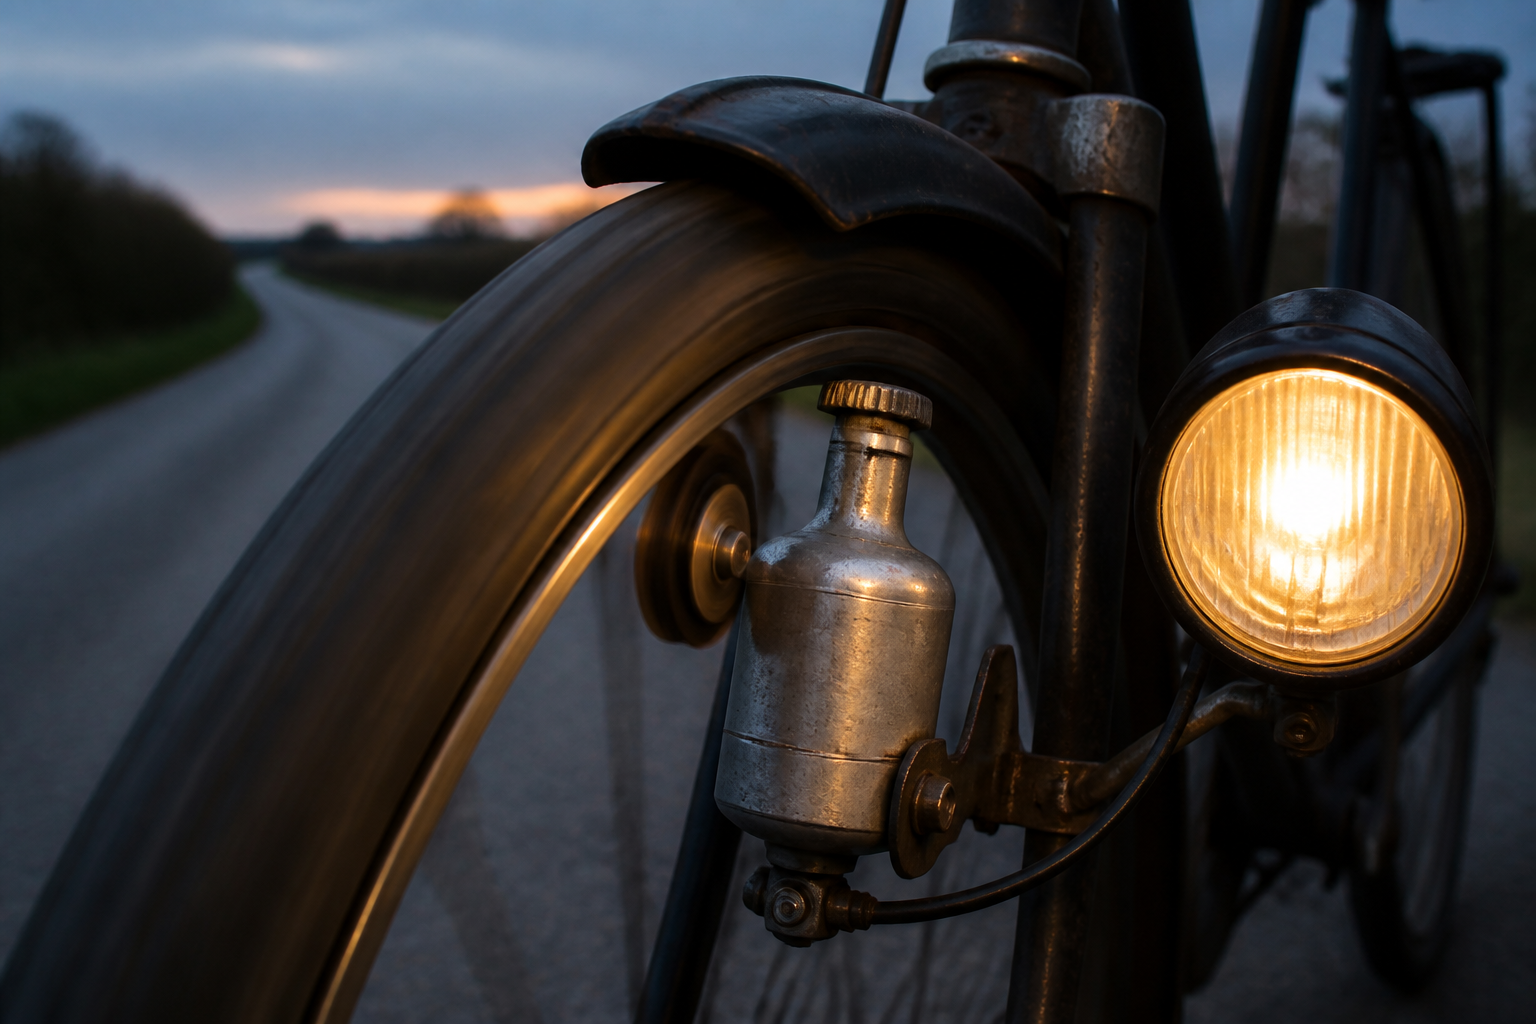
\includegraphics[width=0.58\linewidth]{images/book3/ai/b3-29-bicycle-dynamo.png}

{\small Een fietsdynamo: het wiel draait een magneet in een spoel, de flux door de spoel verandert, en de lamp gaat branden --- de \omterm{thm:b1:induction:faraday}{wet van Faraday} op de fiets.}
\end{omfigure}

\section{Probleem: De fietsdynamo en de luidspreker}

\begin{problem}[{Weekendopgave --- twee elektromechanische omzetters
uit elkaar gehaald: een dynamo die zichzelf regelt, en een luidspreker waarvan de
versterker tegelijk zijn rem is}]
\label{pb:b1:induction:1}

\medskip
\noindent\textbf{Deel I --- De fietsdynamo.}
Een spoel van $N = 300$ windingen met oppervlakte $S = \qty{3.0}{cm^2}$ draait in een
homogeen veld $B = \qty{0.30}{T}$; haar as draagt een rolletje met straal
$r = \qty{1.0}{cm}$ dat tegen de band wordt gedrukt, zodat de spoel met
$\omega = v/r$ draait bij een fietssnelheid $v$. Weerstand van de spoel $r_c = \qty{4.0}{\ohm}$,
\omterm{def:b1:induction:inductance}{zelfinductie} $L = \qty{20}{mH}$; de lamp is een weerstand $R = \qty{12}{\ohm}$.
\begin{enumerate}
  \item Flux door de spoel en geïnduceerde emk als functie van de tijd;
        \omterm{def:b1:wave-propagation:signal}{amplitude} en frequentie bij $v = \qty{18}{km/h}$.
  \item Verwaarloos eerst $L$: effectieve stroom en vermogen in de lamp bij
        \qty{18}{km/h}; is een lamp van ``\qty{6}{V}, \qty{3}{W}'' comfortabel?
  \item Gemiddeld mechanisch vermogen dat de fietser aan de dynamo levert, en
        de bijbehorende kracht op de band (vergelijk met de rolweerstand,
        ongeveer \qty{2}{N}).
  \item Verklaar met de \omterm{thm:b1:induction:faraday}{wet van Lenz} waarom de dynamo tegenwerkt, en waarom een lamp
        die ``gratis'' brandt niet met het energiebehoud in strijd is.
  \item Neem nu $L$ mee: complexe \omterm{def:b1:sinusoidal-impedance:impedance}{impedantie} van de kring; toon aan dat
        de stroomamplitude $I = NBS\omega/\sqrt{(R + r_c)^2 + L^2\omega^2}$ is
        en dat zij bij hoge snelheid verzadigt; geef die limiet en de
        snelheid waarbij zij $70\%$ ervan bereikt.
  \item Wat zou de lamp zonder de \omterm{def:b1:induction:inductance}{zelfinductie} bij
        \qty{54}{km/h} bergaf ontvangen? En met?
  \item Stroom en lampvermogen bij \qty{9}{km/h} en bij \qty{36}{km/h}; becommentarieer
        de zelfregeling.
  \item Echte dynamo's laten een magneet in een vaste spoel draaien. Verandert de
        analyse daardoor? Welk praktisch probleem lost dat op?
  \item Wat doet de lamp wanneer de fiets bij een rood licht stopt,
        en hoe verhelpen moderne lampen dat?
\end{enumerate}

\medskip
\noindent\textbf{Deel II --- De luidspreker.}
Spreekspoel: draadlengte $\ell = \qty{5.0}{m}$ in een radiaal veld $B =
\qty{1.0}{T}$, weerstand $R = \qty{8.0}{\ohm}$, \omterm{def:b1:induction:inductance}{zelfinductie} $L = \qty{0.50}{mH}$;
bewegende massa (spoel en conus) $m = \qty{10}{g}$; stijfheid van de ophanging
$k = \qty{1000}{N/m}$, mechanische demping $h = \qty{1.0}{N.s/m}$. Sinusvormig
regime, \omterm{def:b1:sinusoidal-impedance:complex}{complexe amplitudes}.
\begin{enumerate}[resume]
  \item Kracht op de spoel bij een stroom $i$; tegen-emk bij een snelheid $v$
        (leid beide af, met tekens).
  \item Schrijf de elektrische en de mechanische vergelijking op.
  \item Elimineer $i$ en toon aan dat
        $\underline v = \dfrac{B\ell\,\underline u}{(R + jL\omega)(jm\omega + h + k/j\omega) + B^2\ell^2}$.
  \item Toon aan dat de koppeling bij frequenties waar $L\omega \ll R$ werkt
        als een extra mechanische demping $B^2\ell^2/R$; waarde; resonantie-
        frequentie van de conus en haar \omterm{def:b1:transient-regimes:secondorder}{kwaliteitsfactor} met en zonder
        de elektrische demping.
  \item De versterker levert een $i$ met \omterm{def:b1:wave-propagation:signal}{amplitude} \qty{1.0}{A} bij \qty{1}{kHz}:
        \omterm{def:b1:wave-propagation:signal}{amplitude} van kracht, versnelling, uitwijking en snelheid van de
        conus (massagestuurd regime); \omterm{def:b1:wave-propagation:signal}{amplitude} van de tegen-emk vergeleken met
        $Ri$.
  \item Dezelfde stroom bij de resonantiefrequentie: snelheidsamplitude
        (dempingsgestuurd) en tegen-emk; becommentarieer.
  \item \omterm{thm:b1:dc-circuits:kirchhoff}{Elektrisch vermogen} bij \qty{1}{kHz}; mechanisch vermogen dat in
        $h$ wordt gedissipeerd (opgevat als het geluid en de verliezen in de ophanging); \omterm{def:b1:heat-engines:efficiency}{rendement}.
  \item Waarom is het feit dat de geluidsdruk evenredig is met de versnelling van
        de conus (neem dat aan) de reden dat een massagestuurde conus boven de
        resonantie een vlakke respons geeft?
  \item Waarom moet het veld radiaal zijn, en waarom is een tweeter klein?
  \item Schets de modulus van de \omterm{def:b1:sinusoidal-impedance:impedance}{impedantie} $\underline u/\underline i$ die de
        versterker ziet van \qty{10}{Hz} tot \qty{10}{kHz}: waarde bij lage
        frequentie, bij resonantie (gebruik de dempingsgestuurde snelheid),
        en bij \qty{10}{kHz}.
\end{enumerate}

\medskip
\noindent\textbf{Deel III --- Achterstevoren, en de boekhouding.}
\begin{enumerate}[resume]
  \item Hetzelfde toestel als microfoon: geluid beweegt de conus met
        $v = \qty{1.0}{mm/s}$; nullastspanning.
  \item Belast met $R_L = \qty{600}{\ohm}$: stroom, en de remkracht
        op de conus; toon aan dat de microfoon vermogen uit het geluid haalt
        via een effectieve demping $B^2\ell^2/(R + R_L)$.
  \item De spoel is op een aluminium cilindertje gewikkeld (de spoeldrager), een
        gesloten winding met lengte \qty{0.10}{m} en weerstand \qty{1.0}{m\ohm}:
        de demping die zij toevoegt; waarom spoeldragers een spleet krijgen.
  \item Tik tegen de conus van een luidspreker waarvan de klemmen open staan, en
        daarna van een waarvan de klemmen zijn kortgesloten: welke van de twee natrilt langer,
        en waarom?
  \item Schrijf de energiebalans van de luidspreker over één periode in
        stationair regime op, en benoem elke term.
  \item Vat samen: voor elk toestel de gebruikte wet en de twee getallen
        die het onthouden waard zijn.
\end{enumerate}
\end{problem}
